\spacing{1.25}
\vspace{-5mm}
En este cap\'itulo se presentan y discuten los resultados obtenidos de la componente mu\'onica de la distribuci\'on lateral de cascadas atmosf\'ericas a partir de simulaciones con AIRES. Se realiza un ajuste de la distribuci\'on lateral de muones a una funci\'on de tipo NKG modificada, y se grafican los par\'ametros del ajuste en funci\'on de la energ\'ia primaria. Se comparan los par\'ametros obtenidos como resultado de distintas part\'iculas primarias, diferentes modelos de interacciones hadr\'onicas y distintos \'angulos de incidencia. Tambi\'en se calcula un aproximado de la cantidad de muones de cascadas atmosf\'ericas que podr\'ian observarse en HAWC.

\section{Distribuci\'on lateral de muones}	
La distribuci\'on lateral de muones $\rho_{\mu}(r)$ contiene informaci\'on sobre la energ\'ia primaria $E_0$, la masa primaria A, el \'angulo zenital $\theta$ y la edad de la cascada \cite{Albrecht2021}. Se simularon cascadas atmosf\'ericas con $12 < \log(E_0/\text{eV}) < 14$, A$=1$ (protones), A$=56$ (n\'ucleos de hierro) y $0^{\circ} < \theta \leq 45^{\circ}$; limitando el estudio a eventos cuyos muones puedan ser detectados por el observatorio HAWC. De acuerdo a la condici\'on necesaria para que los muones produzcan radiaci\'on Cherenkov en el agua
	\begin{align}
	\beta_{\mu} > \frac{1}{n_{\text{agua}}},
	\end{align}
donde $\beta_{\mu}=v_{\mu}/c$ es la velocidad del mu\'on relativa a la rapidez de la luz y $n_{\text{agua}}$ es el \'indice de refracci\'on del agua, la energ\'ia umbral para que los muones puedan detectarse en HAWC es $E_{th}\approx 159.80$ MeV, por lo que se han filtrado los resultados de las simulaciones tomando en cuenta solamente muones con energ\'ias $E_{\mu} > E_{th}$. \\
	
En la Figura \ref{fig:lateraldist} se presentan las distribuciones laterales obtenidas para tres energ\'ias primarias: $10^{12}$, $10^{13}$ y $10^{14}$ eV. Las cascadas fueron iniciadas por protones y n\'ucleos de hierro con un \'angulo zenital de incidencia $\theta$ entre 0 y 45$^{\circ}$. En t\'erminos generales se observa el comportamiento esperado: la densidad de muones decrece con la distancia radial $R$, es decir que al estar m\'as lejos del eje de la cascada se encuentran menos muones; tambi\'en los valores de densidad de muones aumentan al incrementar la energ\'ia primaria (de izquierda a derecha en la figura). Por otro lado, es notable que en el rango radial que se est\'a considerando ($R<300$ m) a bajas energ\'ias las cascadas iniciadas por protones presentan m\'as muones que las iniciadas por n\'ucleos de hierro, sin embargo a medida que la energ\'ia aumenta los resultados de ambas se incerceptan, de manera que a 100 TeV la curva del hierro se encuentra por encima de la de un prot\'on en casi todo el rango de $R$.\\
		\begin{figure}[] 
	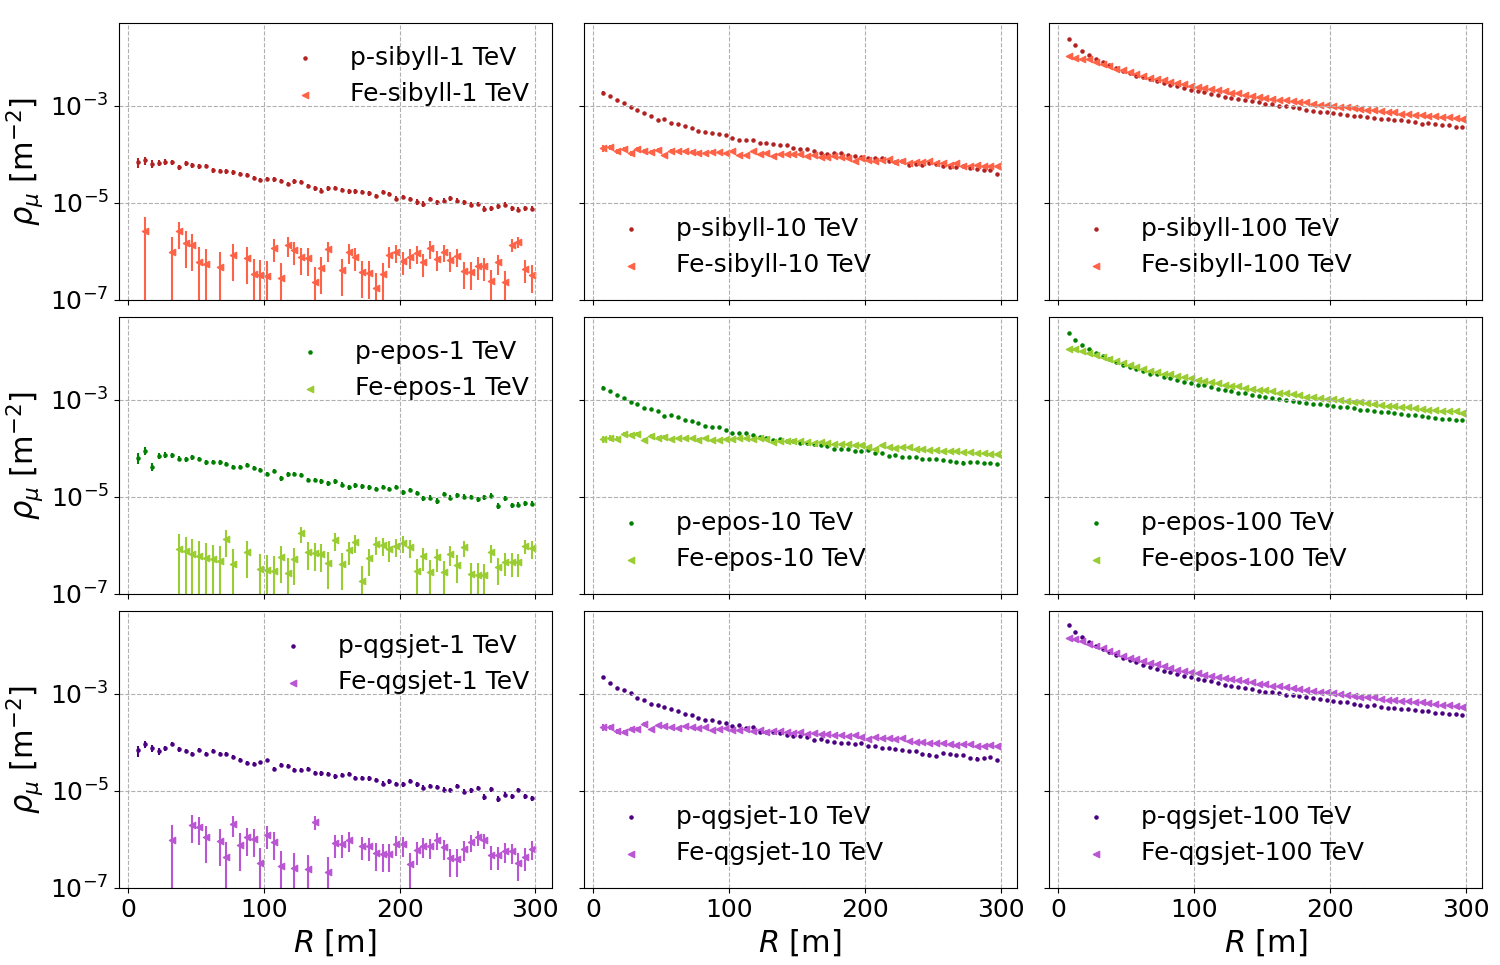
\includegraphics[width=\textwidth]{Figuras/lateraldist}
	\caption{Densidad de muones en funci\'on de la distancia $R$ a partir del eje de la cascada. Se muestran resultados de cascadas de protones (p) y n\'ucleos de hierro (Fe) con tres energ\'ias primarias (aumentando de izquierda a derecha: 1, 10 y 100 TeV) y de los tres modelos de interacciones hadr\'onicas de altas energ\'ias (de arriba a abajo: Sibyll 2.3d, EPOS-LHC y QGSJETII-04). Las distribuciones para las energ\'ias intermedias se encuentran en el Ap\'endice A.}
	\label{fig:lateraldist}
	\end{figure}	

Adicionalmente, las distribuciones laterales de muones obtenidas se han contrastado con resultados publicados por otros autores que han realizado las simulaciones con el programa CORSIKA; esto permite comprobar de cierta manera que los resultados que se han obtenido con AIRES son de hecho razonables y similares a los que se consiguen con CORSIKA. Dichas comparaciones se presentan en las Figuras \ref{fig:comparacion_otros} y \ref{fig:comparacion_parsons} superponiendo las distribuciones laterales de este trabajo (designadas con el nombre AIRES en las gr\'aficas) con las de Gupta et al. (2005), Mitchell et al. (2019) y Parsons y Schoorlemmer (2019), que realizaron simulaciones con caracter\'isticas similares, aunque con algunas diferencias en el \'angulo zenital, la altura del suelo y la energ\'ia umbral de los muones.\\

En la primera gr\'afica (Figura \ref{fig:comparacion_otros}) se presentan resultados utilizando el modelo QGSJET. Los resultados de Gupta et al. (l\'inea negra con marcadores circulares vac\'ios) corresponden a cascadas de 300 TeV \cite{Gupta2005} que, al tener mayor energ\'ia primaria, se encuentran por encima de la curva de AIRES de 100 TeV, la energ\'ia m\'axima considerada en este trabajo. Adem\'as se muestran resultados de 10 TeV  de Mitchell et al. \cite{Mitchell2019} (l\'inea gris con marcadores triangulares vac\'ios) donde se observan menores densidades que en los resultados de AIRES para la misma energ\'ia primaria, lo cual se atribuye al \'angulo zenital de incidencia de las cascadas, que en \cite{Mitchell2019} es $20^{\circ}$ mientras que la curva de AIRES corresponde a cascadas con \'angulos zenitales entre 0 y $20^{\circ}$, a la energ\'ia umbral de 10 GeV y la altura menor (1800 m frente a 4100 m de HAWC).\\
	\begin{figure}[] 
	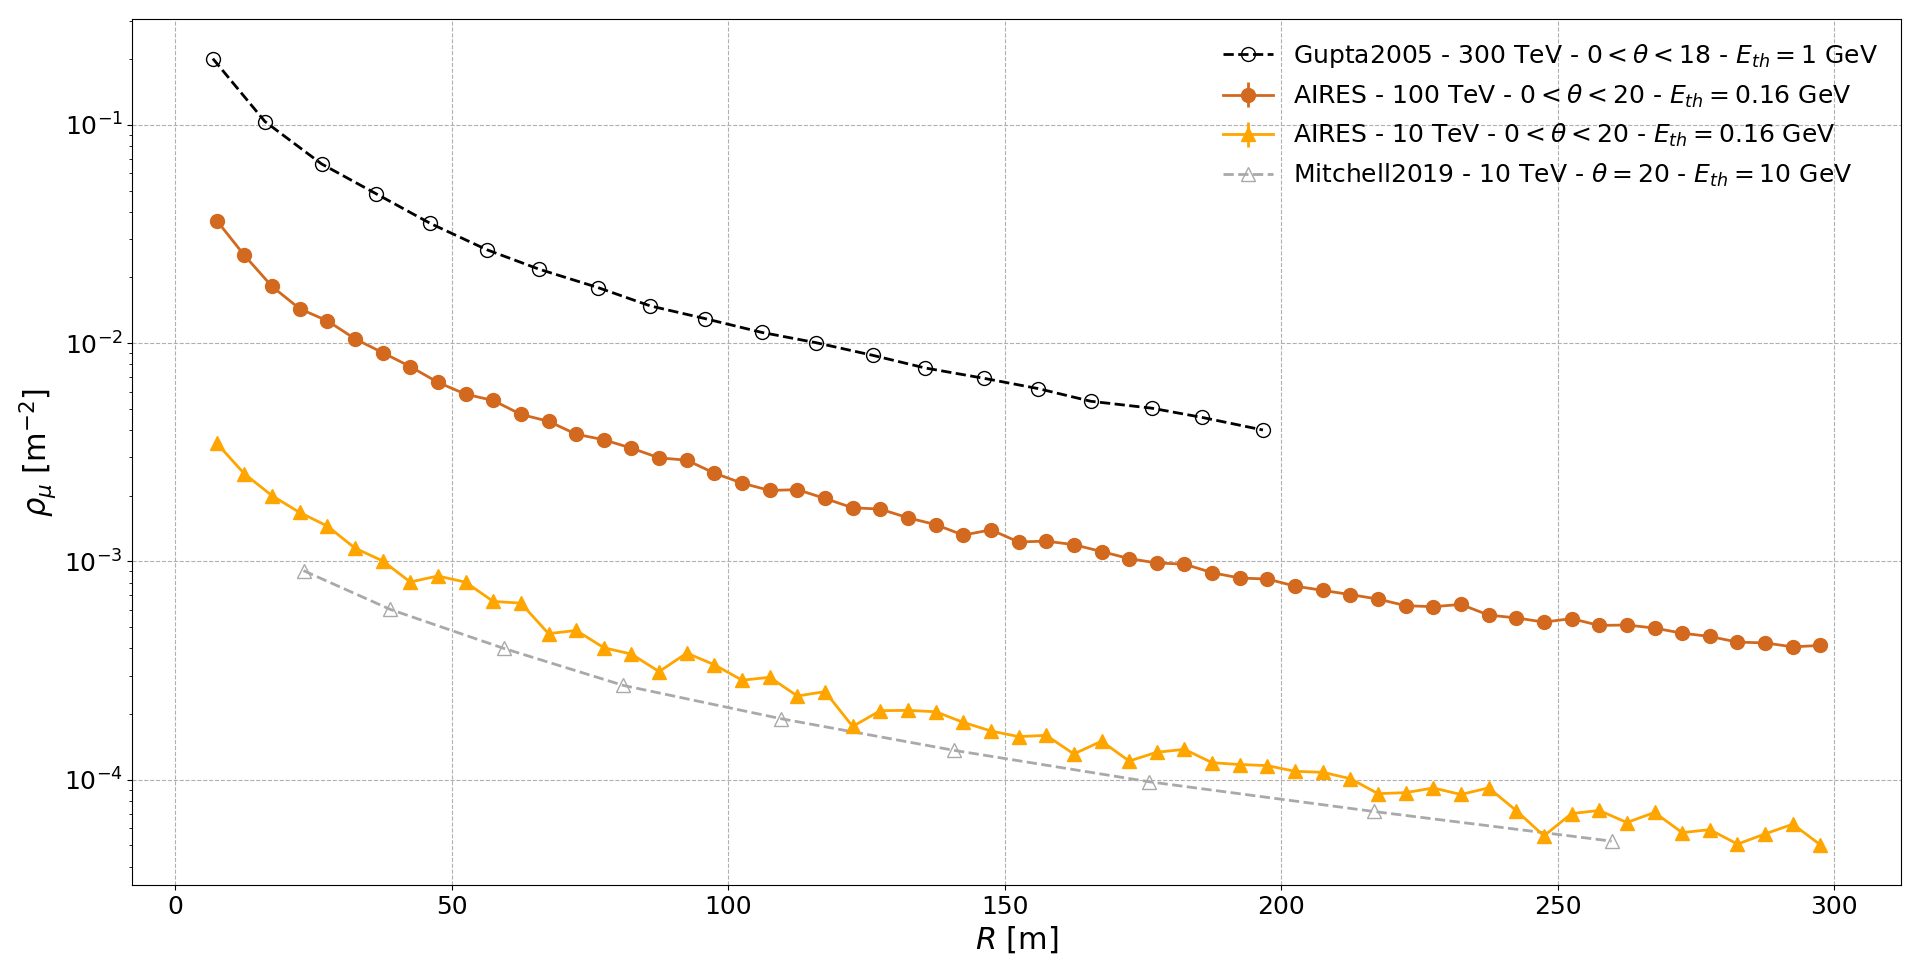
\includegraphics[width=\textwidth]{Figuras/comparacion_otros}
	\caption{Comparaci\'on de los resultados obtenidos con AIRES (l\'ineas naranja) de la distribuci\'on lateral de muones a 100 y 10 TeV con resultados de otros autores: Gupta et al. (2005) \cite{Gupta2005} y Mitchell et al. (2019) \cite{Mitchell2019}, a 300 TeV y 10 TeV, respectivamente. La discrepancia en las curvas de 10 TeV se atribuye al \'angulo $\theta$ de incidencia de las cascadas simuladas y a la altura de observaci\'on.}
	\label{fig:comparacion_otros}
	\end{figure}	
	
Igualmente, en la Figura \ref{fig:comparacion_parsons} se muestran los resultados de Parsons y Schoorlemmer (2019), cuyas simulaciones est\'an en el mismo rango de energ\'ia y en la misma ubicaci\'on (el observatorio HAWC) \cite{Parsons2019} que las de AIRES. En este caso, las graficas reflejan resultados obtenidos con el modelo EPOS-LHC. Se observa que las densidades de muones de \cite{Parsons2019} son m\'as altas con respecto a las del presente trabajo. Similar al caso anterior, esta discrepancia entre resultados de cascadas con la misma energ\'ia (y a la misma altura) se explica por el \'angulo de incidencia, ya que en la publicaci\'on han simulado con CORSIKA cascadas totalmente verticales ($\theta=0$), de las cuales llegan al suelo una mayor cantidad de part\'iculas.\\
	\begin{figure}[] 
	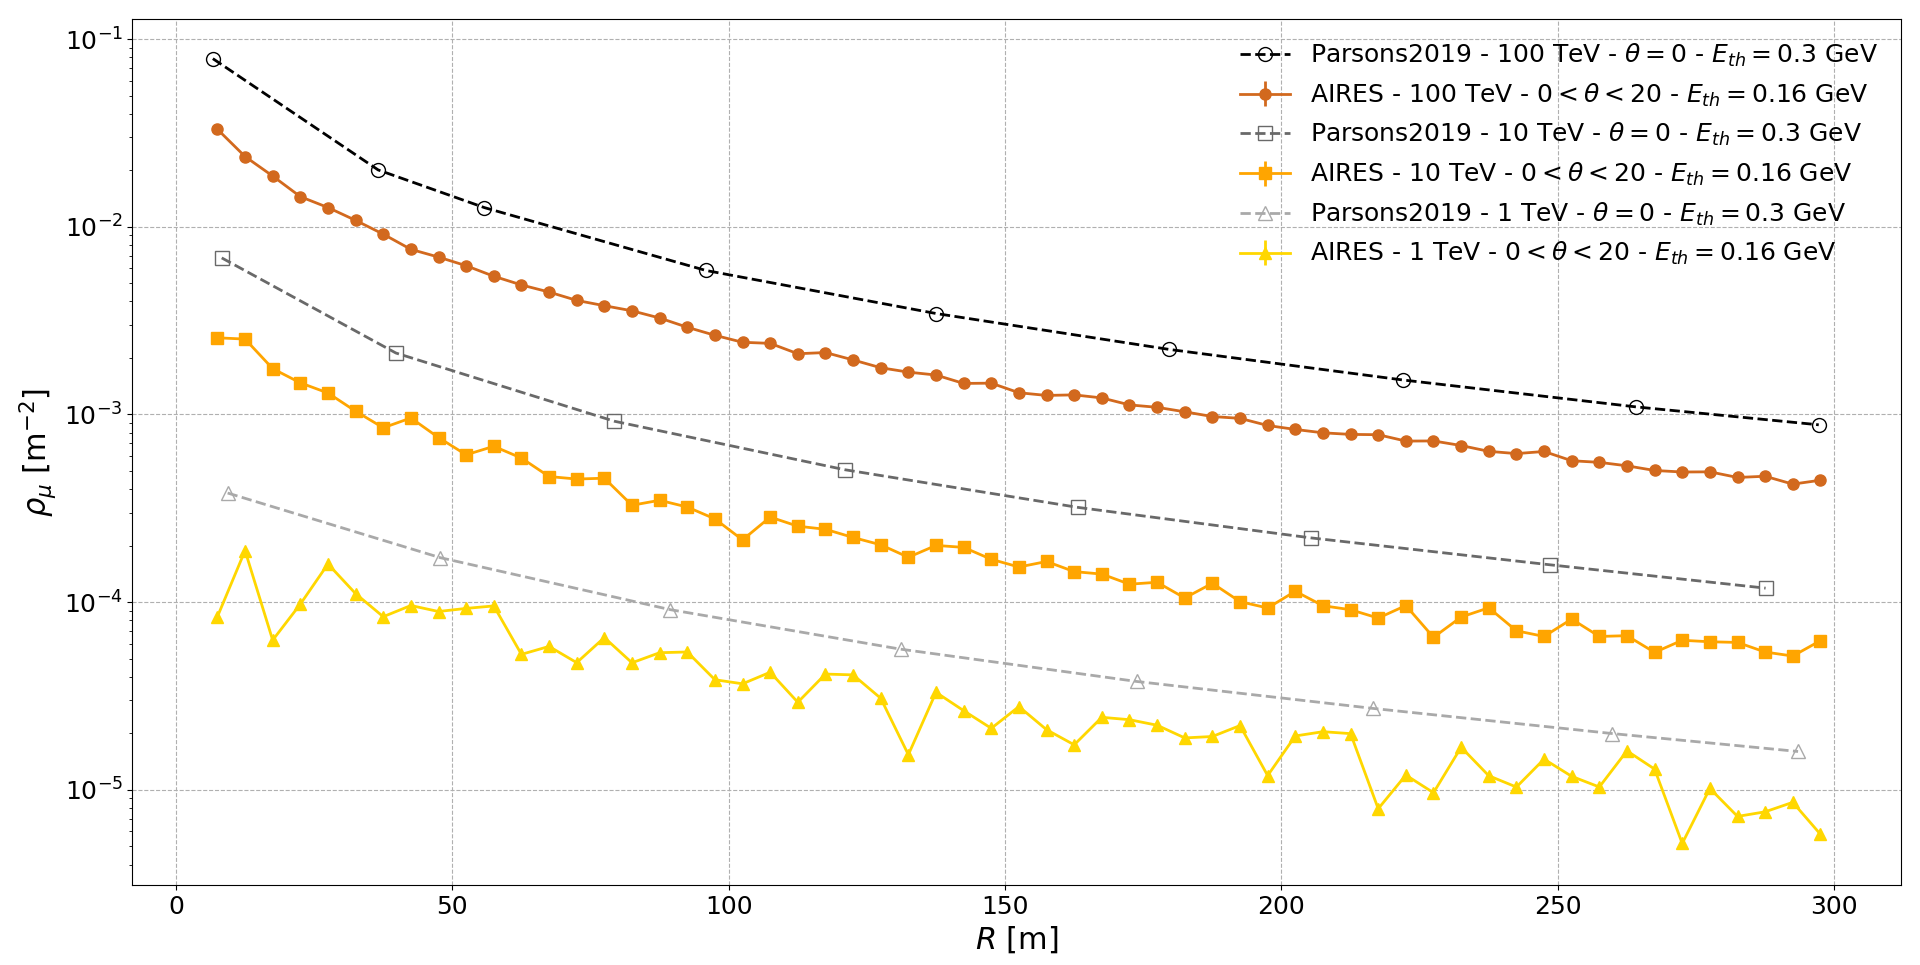
\includegraphics[width=\textwidth]{Figuras/comparacion_parsons2019}
	\caption{Comparaci\'on de los resultados obtenidos con AIRES (l\'ineas naranja) de la distribuci\'on lateral de muones a 100, 10 y 1 TeV con resultados de Parsons y Schoorlemmer (2019) \cite{Parsons2019} con las mismas energ\'ias. Las discrepancias se atribuyen al \'angulo $\theta$ de incidencia de las cascadas.}
	\label{fig:comparacion_parsons}
	\end{figure}	
	
	\subsection{Ajustes a una funci\'on de tipo NKG}
%	\ccnote{Presentaci\'on de la funci\'on (cita a Malone2018, ah\'i se usa para ajustar la carga efectiva y estimar el radio \'optimo en HAWC). Interpretaci\'on de los par\'ametros libres.}
	Cada una de las distribuciones laterales de muones obtenidas se ajust\'o a una funci\'on de tipo NKG modificada, utilizada por la colaboraci\'on HAWC para ajustar la distribuci\'on lateral de la carga efectiva en cascadas iniciadas por rayos gamma	\cite{Malone2018} y por rayos c\'osmicos \cite{Morales-Soto2019}:
	\begin{align} \label{eq:nkg}
	\rho_{\mu}(r) = A \qty(\frac{r}{r_M})^{s-3}\qty(1+\frac{r}{r_M})^{s-4.5},
	\end{align}
	donde $r_M$ es el radio de \textit{Moli\`ere} a la altura de HAWC (124.21 m), mientras que $A$ y $s$ son par\'ametros libres del ajuste. El par\'ametro $A$ es una amplitud (o constante de normalizaci\'on) que est\'a relacionada con el n\'umero de part\'iculas ($N_{\mu}$ en este caso) en un \'area determinada, y $s$ est\'a relacionado con la edad de la cascada, es decir la etapa del desarrollo de la misma; un valor de $s<1$ indica que la cascada a\'un no alcanza su m\'aximo, en $s=1$ la cascada est\'a en el m\'aximo y en $s>1$ la cascada ya tuvo su m\'aximo y se est\'a atenuando. En la Figura \ref{fig:lateraldist_wfits} se muestran los datos de tres energ\'ias primarias junto con las curvas resultantes del ajuste. En las siguientes secciones se presentan los par\'ametros $A$ y $s$ en funci\'on de la energ\'ia primaria de las cascadas.\\
		\begin{figure}[] 
		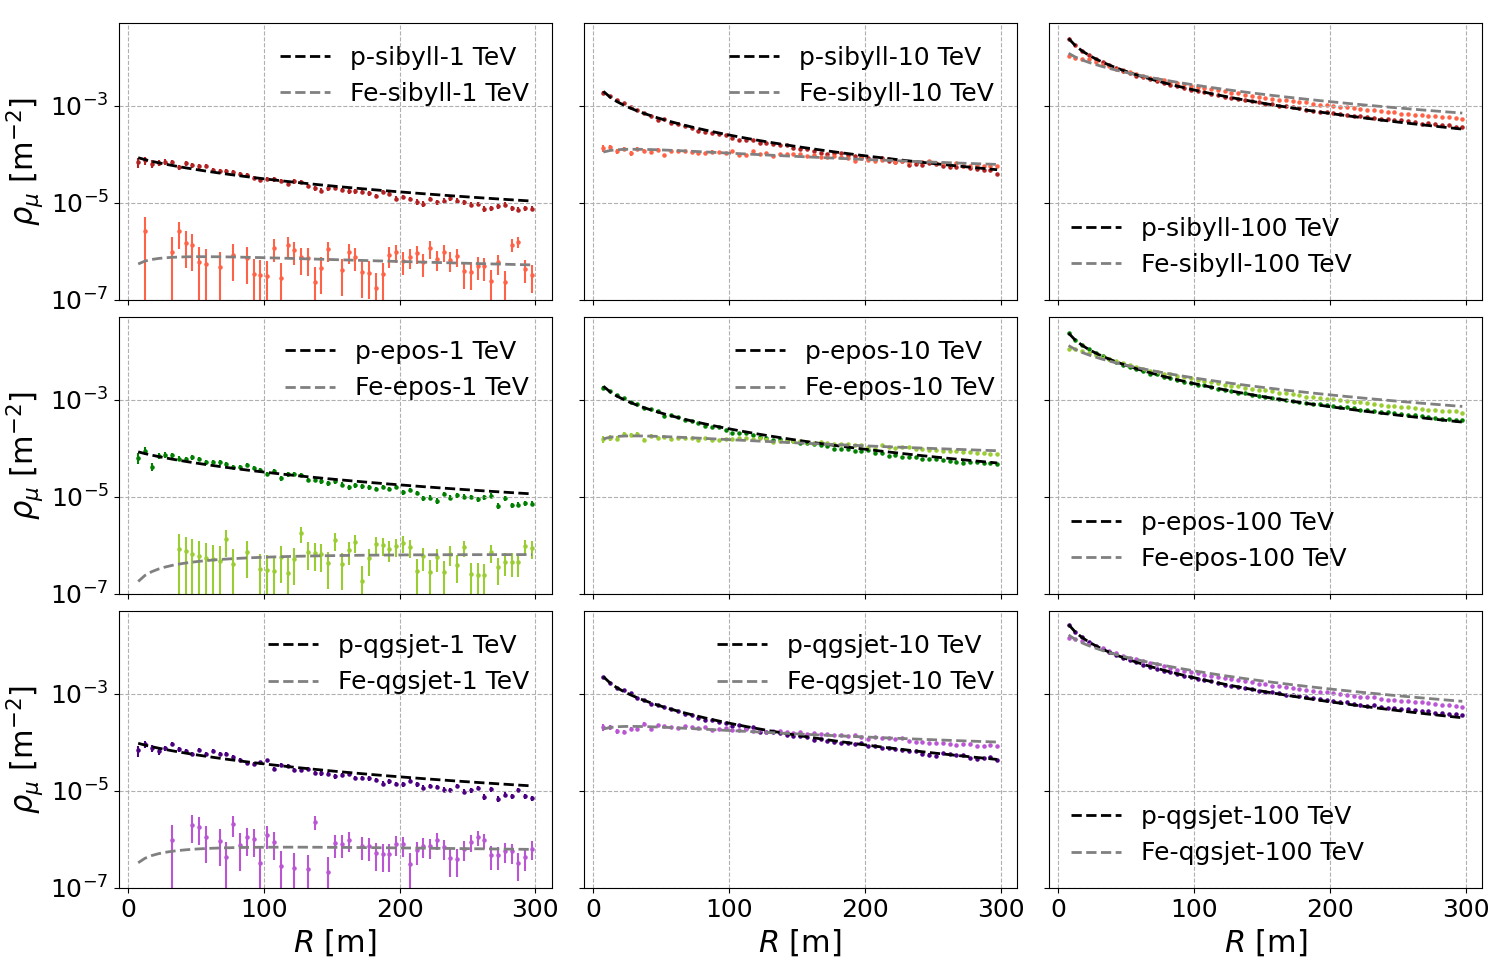
\includegraphics[width=\textwidth]{Figuras/lateraldist_wfits}
		\caption{Resultados de la Figura \ref{fig:lateraldist} junto con la curva resultante del ajuste a la funci\'on $\rho_{\mu}(r)$ de tipo NKG modificada (l\'ineas discontinuas) de la ecuaci\'on (\ref{eq:nkg}). Las distribuciones con sus respectivos ajustes para las energ\'ias intermedias se encuentran en el Ap\'endice A.}
		\label{fig:lateraldist_wfits}
		\end{figure}
		
%	\ccnote{Descripci\'on del ajuste: $\chi ^2$. Puedo poner una figura, o s\'olo mencionar los rangos.}
		
\section{Par\'ametros del ajuste}
Con los par\'ametros $A$ y $s$ se caracterizan las distribuciones laterales y su evoluci\'on con la energ\'ia primaria. En esta secci\'on se explora dicha evoluci\'on desde diferentes perspectivas: primero se eval\'ua la influencia de los modelos de interacciones hadr\'onicas utilizados en las simulaciones, luego se comparan los resultados de cascadas con distinta part\'icula primaria y por \'ultimo se explica el efecto del \'angulo zenital de incidencia del rayo c\'osmico. \\

En t\'erminos generales, lo que se aprecia en los resultados es que $A$ es un par\'ametro que crece con la energ\'ia primaria, es decir que a mayor energ\'ia una cascada atmosf\'erica contiene m\'as muones debido a que hay m\'as energ\'ia disponible en su componente hadr\'onica. Por su parte el par\'ametro $s$ muestra el comportamiento opuesto, disminuyendo con $E$, dando a entender que a medida aumenta la energ\'ia primaria se observan cascadas m\'as ``j\'ovenes'', en concordancia con que la profundidad del m\'aximo $X_{\text{max}}$ es mayor.

	\subsection{Modelos de interacciones hadr\'onicas}
%	\ccnote{comparaci\'on entre A y s obtenidos con cada modelo (Figuras \ref{fig:models_nkgA} y \ref{fig:models_nkgs}). Son iguales jeje.}
	
	Los tres modelos de interacciones hadr\'onicas de altas energ\'ias utilizados (Sibyll 2.3d, EPOS-LHC y QGSJETII-04) abordan los aspectos de las interacciones de diferente manera. En particular, los aspectos de las interacciones hadr\'onicas que impactan m\'as directamente el desarrollo de las cascadas atmosf\'ericas son la secci\'on eficaz, la multiplicidad y la inelasticidad; las diferencias entre los modelos son debidas principalmente a las extrapolaciones que realizan a interacciones p-aire y $\pi$-aire a partir de datos experimentales de interacciones p-p \cite{Pierog2018}. La intenci\'on de comparar los resultados de diferentes modelos, en este caso, es evaluar la distribuci\'on lateral de la componente mu\'onica como una observable con la cual se pueda discriminar entre ellos.\\
		\begin{figure} []
		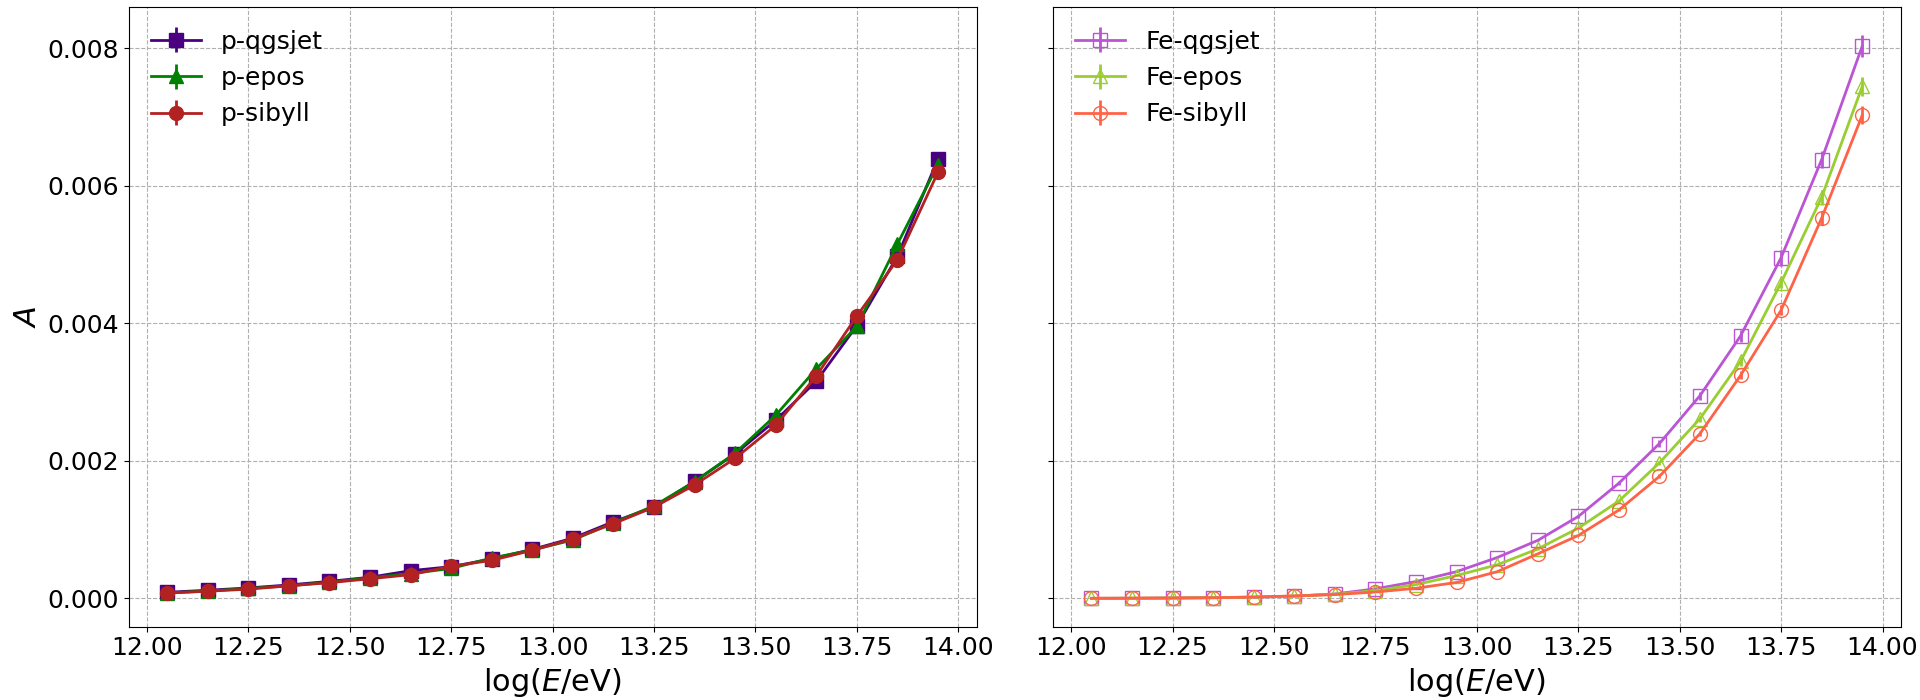
\includegraphics[width=\textwidth]{Figuras/models_nkgA}
		\caption{Resultados del par\'ametro $A$ obtenido en el ajuste de la distribuci\'on lateral simulada a la ecuaci\'on (\ref{eq:nkg}). Se superponen los resultados de los tres modelos hadr\'onicos para cascadas de protones (izquierda) y hierro (derecha), observando que en el primer caso no se presentan diferencias significativas entre ellos, mientras de para Fe es posible apreciar peque\~{n}as diferencias a partir de $10^{13}$ eV.}
		\label{fig:models_nkgA}
		\end{figure}	
		
		\begin{figure} []
		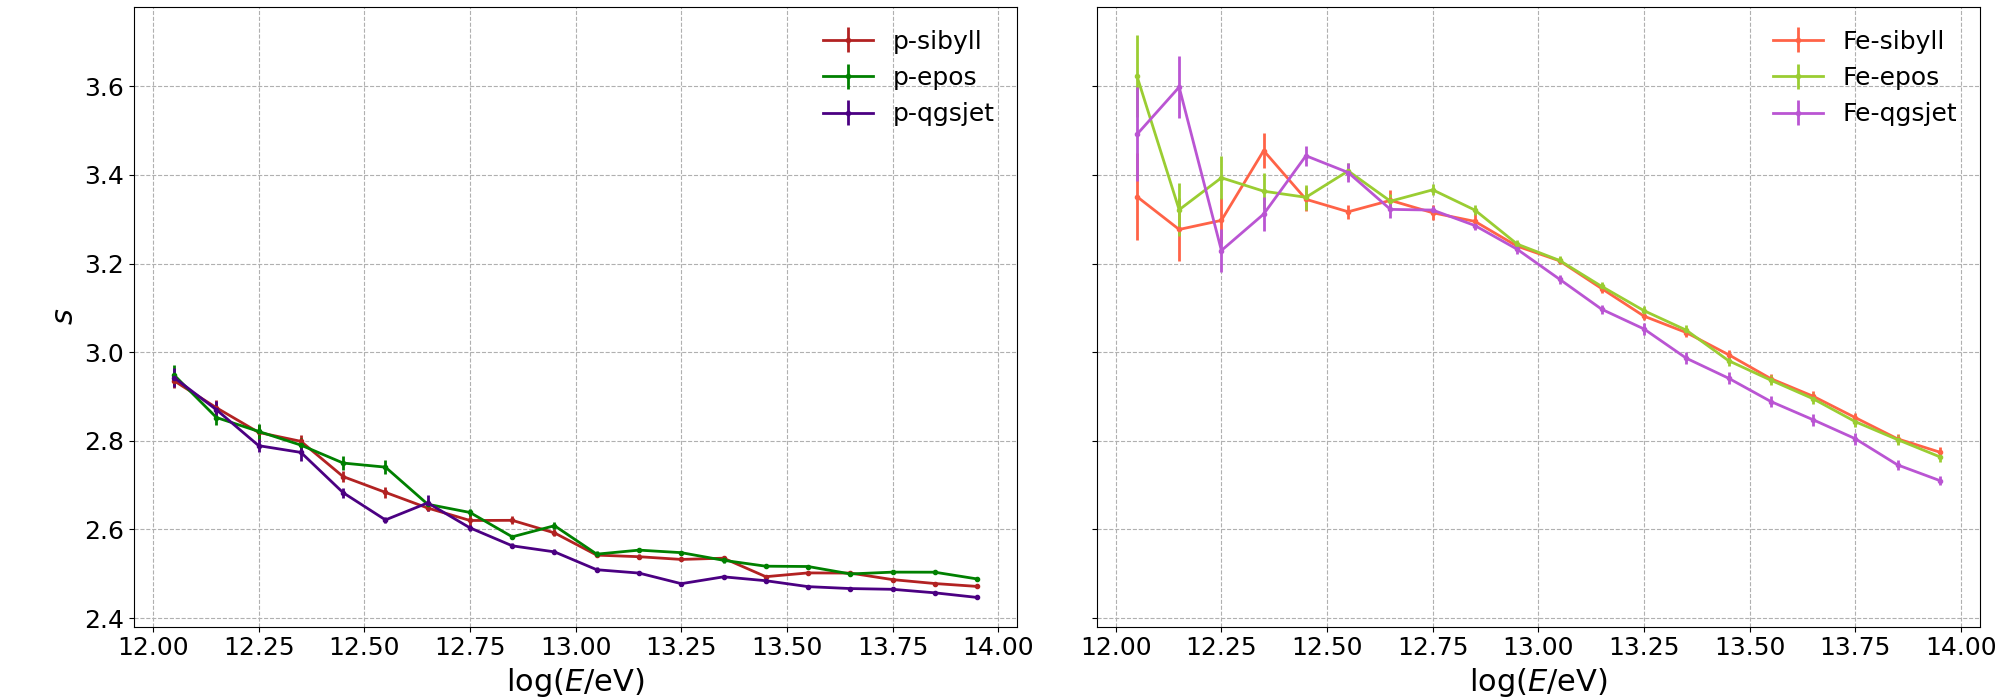
\includegraphics[width=\textwidth]{Figuras/models_nkgs}
		\caption{Resultados del par\'ametro $s$ obtenido en el ajuste de la distribuci\'on lateral simulada a la ecuaci\'on (\ref{eq:nkg}). Se superponen los resultados de los tres modelos hadr\'onicos para cascadas de protones (izquierda) y hierro (derecha). A energ\'ias $>10^{13}$ eV la curva del modelo QGSJETII-04 se aprecia ligeramente por debajo de los otros dos.}  
		\label{fig:models_nkgs}
		\end{figure}	
		
		\begin{figure} []
		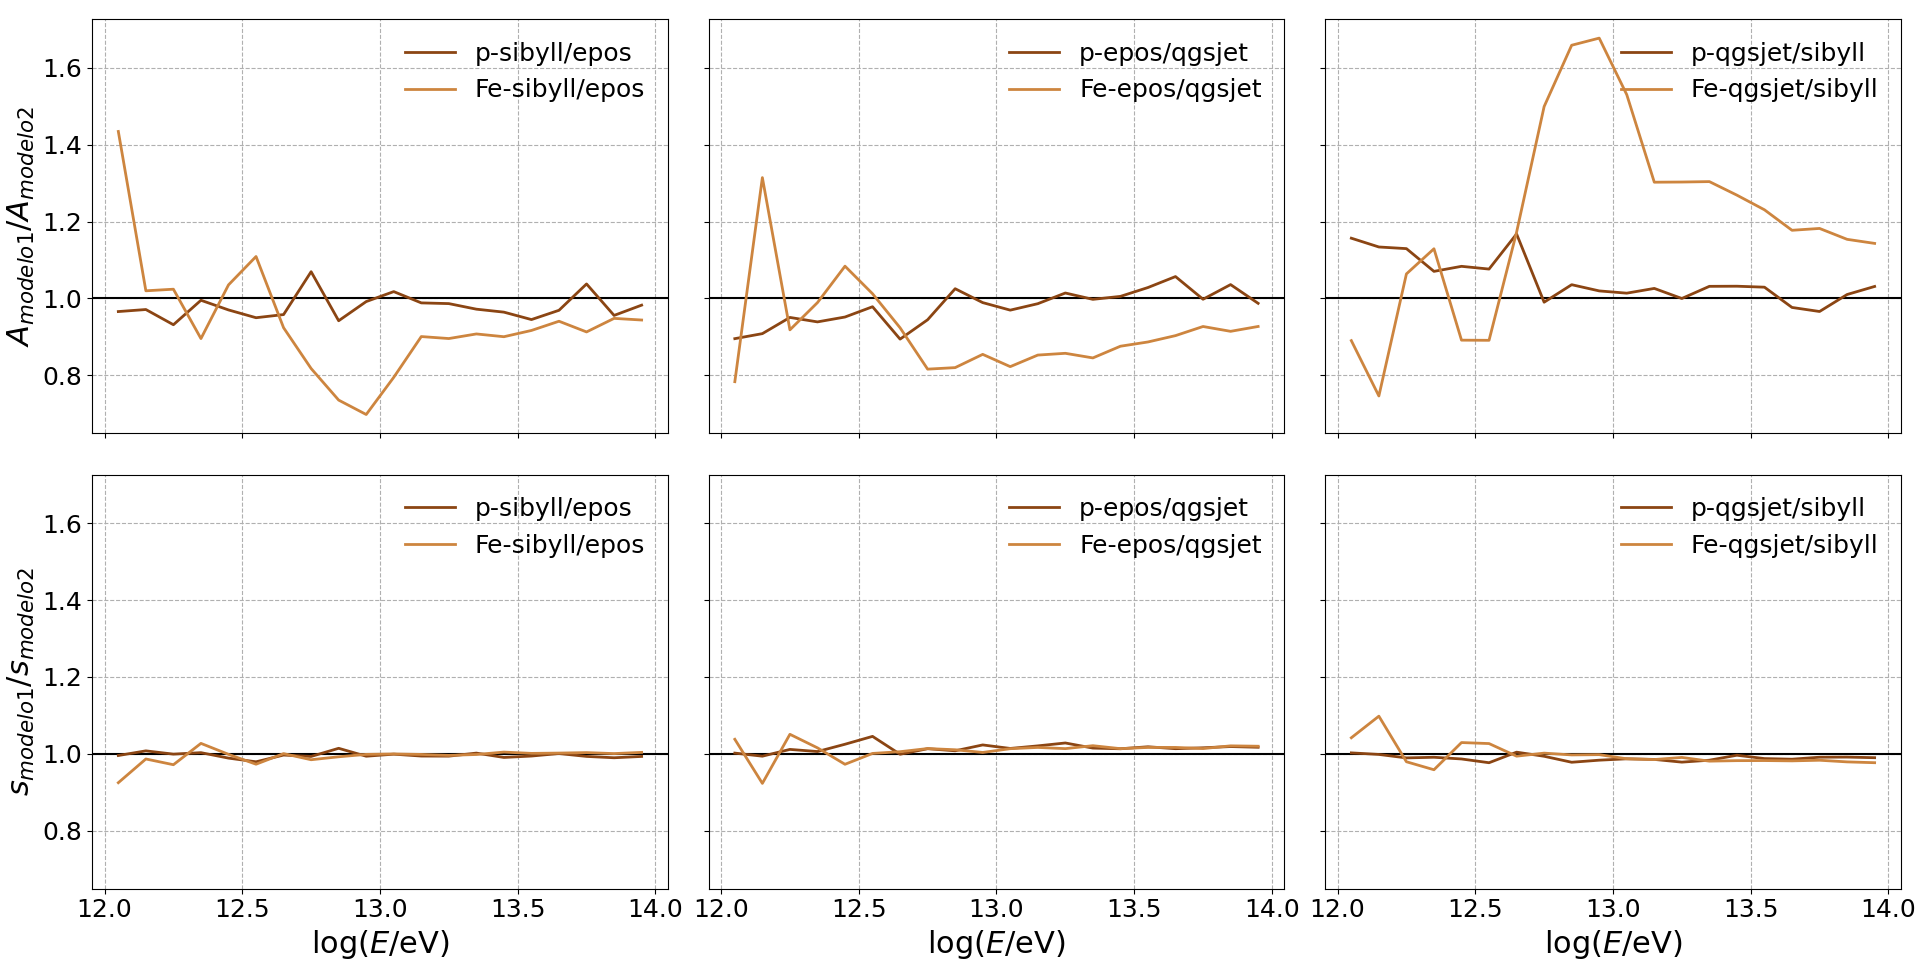
\includegraphics[width=\textwidth]{Figuras/models_ratios}
		\caption{Razones entre los resultados de los diferentes modelos de interacciones hadr\'onicas. Se observa que las mayores diferencias corresponden a las cascadas iniciadas por n\'ucleos de hierro.}
		\label{fig:models_ratios}
		\end{figure}
	
				
	En las Figuras \ref{fig:models_nkgA} y \ref{fig:models_nkgs} se han superpuesto los resultados de los modelos para los par\'ametros $A$ y $s$, respectivamente, en funci\'on de la energ\'ia primaria. En las cascadas iniciadas por protones, el par\'ametro $A$ obtenido con los tres modelos coincide muy bien, de manera que las tres curvas son pr\'acticamente indistinguibles; el caso del par\'ametro $s$ es muy parecido. Por otro lado, para las cascadas producidas por Fe los resultados de $A$ tambi\'en est\'an bastante cercanos, aunque s\'i se observa que la curvas se van separando a medida que aumenta la energ\'ia primaria; para el par\'ametro $s$ las incertezas a bajas energ\'ias son bastante grandes, de manera que no se aprecian diferencias, sin embargo al incrementar la energ\'ia la curva de QGSJET se observa ligeramente por debajo que las de los otros modelos.\\
		
		Para visualizar m\'as claramente las diferencias entre los resultados de los tres modelos de interacciones hadr\'onicas para los par\'ametros del ajuste, en la Figura \ref{fig:models_ratios} se grafica la raz\'on entre los valores obtenidos con cada uno de ellos. En las cascadas de protones las m\'aximas diferencias son del 17\% entre QGSJET y SIBYLL en el par\'ametro $A$, y 5\% entre QGSJET y EPOS en el par\'ametro $s$. Por otro lado, se observan que en las cascadas de hierro las m\'aximas diferencias est\'an entre los modelos QGSJET y SIBYLL, con 68\% y 10\% en los par\'ametros $A$ y $s$, respectivamente.

%	Observando las diferencias entre los modelos remarcadas en la Figura \ccnote{poner figura de las razones de una} 
%	
%		\ccnote{Porcentajes de diferencias. Mencionar posibles causas, de acuerdo a las caracter\'isticas principales de cada modelo.}
		
		
	\subsection{Composici\'on primaria}	
	Distinguiendo entre cascadas de la misma energ\'ia iniciadas por protones e iniciadas por n\'ucleos de hierro, se espera que en las \'ultimas se produzcan mayor cantidad de muones, de acuerdo a la ecuaci\'on (\ref{eq:NmuA}). Sin embargo, en los resultados del par\'ametro $A$, relacionado con $N_{\mu}$, se observa que las cascadas de protones contienen m\'as muones hasta una energ\'ia entre $\approx 25$ y $40$ TeV, a partir de la cual la curva de las cascadas de hierro indica una mayor cantidad de muones. Esto se atribuye a las distancias consideradas en estas simulaciones ($R < 300$ m), ya que si bien las cascadas iniciadas por Fe producen m\'as muones en total, \'estas se extienden m\'as lateralmente debido a la distribuci\'on de la energ\'ia primaria entre los nucleones que participan en las interacciones, por lo que la mayor\'ia de muones estar\'ian a mayores distancias del eje.\\
%	\ccnote{revisar si esto es cierto, ahorita s\'olo es mi intuici\'on}.
			
	Por otro lado, en los resultados del par\'ametro $s$ es evidente la distinci\'on entre cascadas iniciadas por una part\'icula ligera y una pesada. Los mayores valores de $s$ para cascadas de Fe en todo el intervalo de energ\'ia indican cascadas m\'as ``viejas'', ya que \'estas se desarrollan m\'as r\'apido con respecto a las de protones, alcanzando su m\'aximo a menores profundidades atmosf\'ericas, como se expresa en la ecuaci\'on (\ref{eq:XmaxA}). Adem\'as se puede ver que las curvas tienen formas distintas, ya que la de protones tiene una pendiente menor, disminuyendo m\'as lento con la energ\'ia que las cascadas de hierro.\\
%	\ccnote{no s\'e a qu\'e se puede deber esto.}
		\begin{figure} [h]
		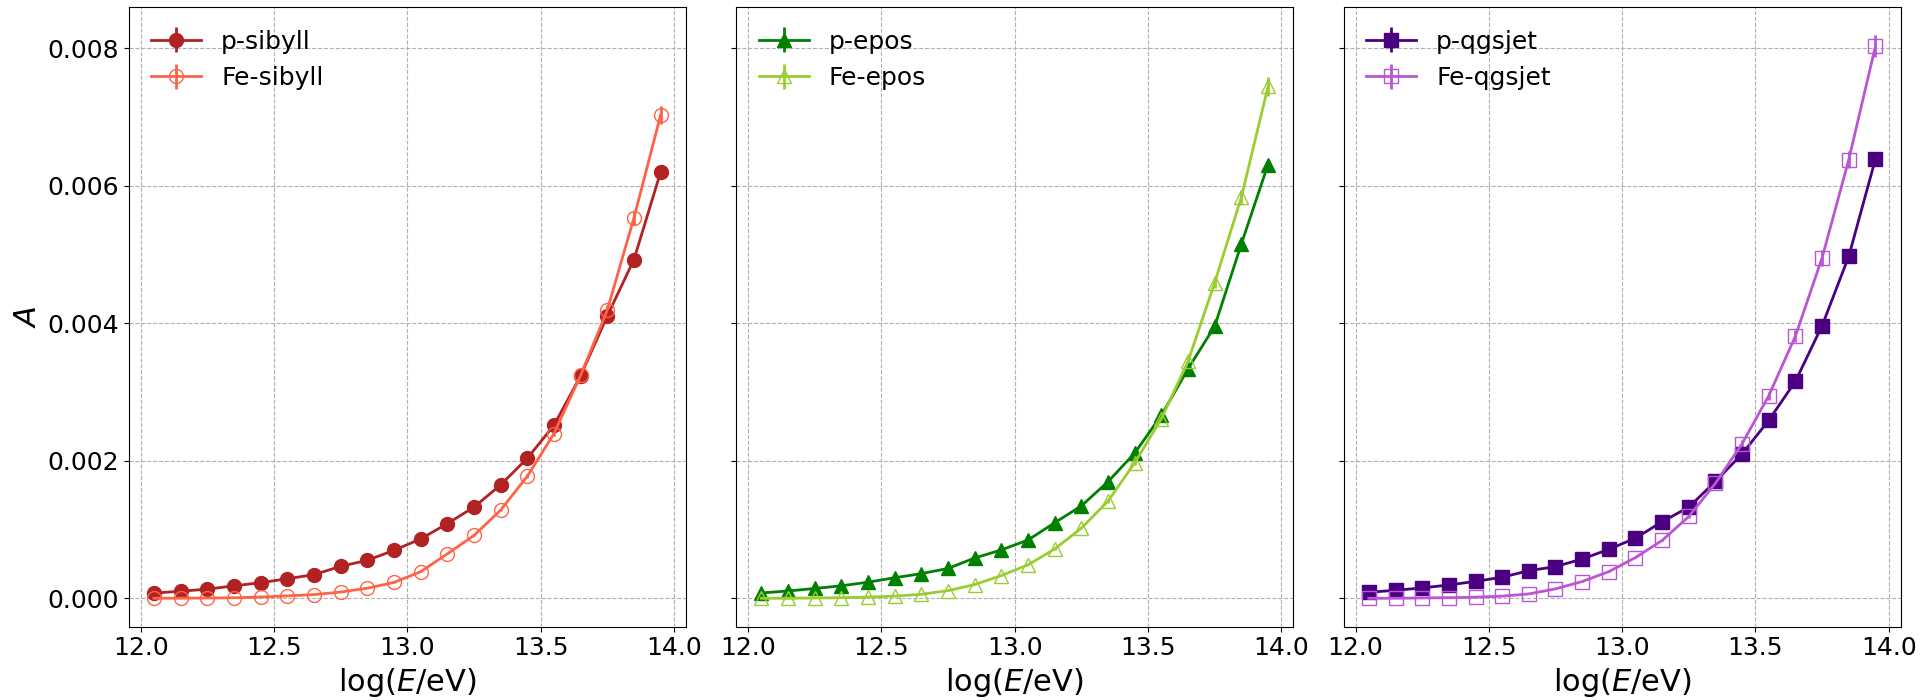
\includegraphics[width=\textwidth]{Figuras/composition_nkgA}
		\caption{Se superponen los resultados del par\'ametro $A$ para cascadas de protones y hierro, con el fin de observar el efecto de la masa de la part\'icula primaria. A bajas energ\'ias se observa la curva de p sobre la de Fe, sugiriendo un mayor n\'umero de muones a las distancias radiales consideradas.}
		\label{fig:composition_nkgA}
		\end{figure}		
		
		\begin{figure} [h]
		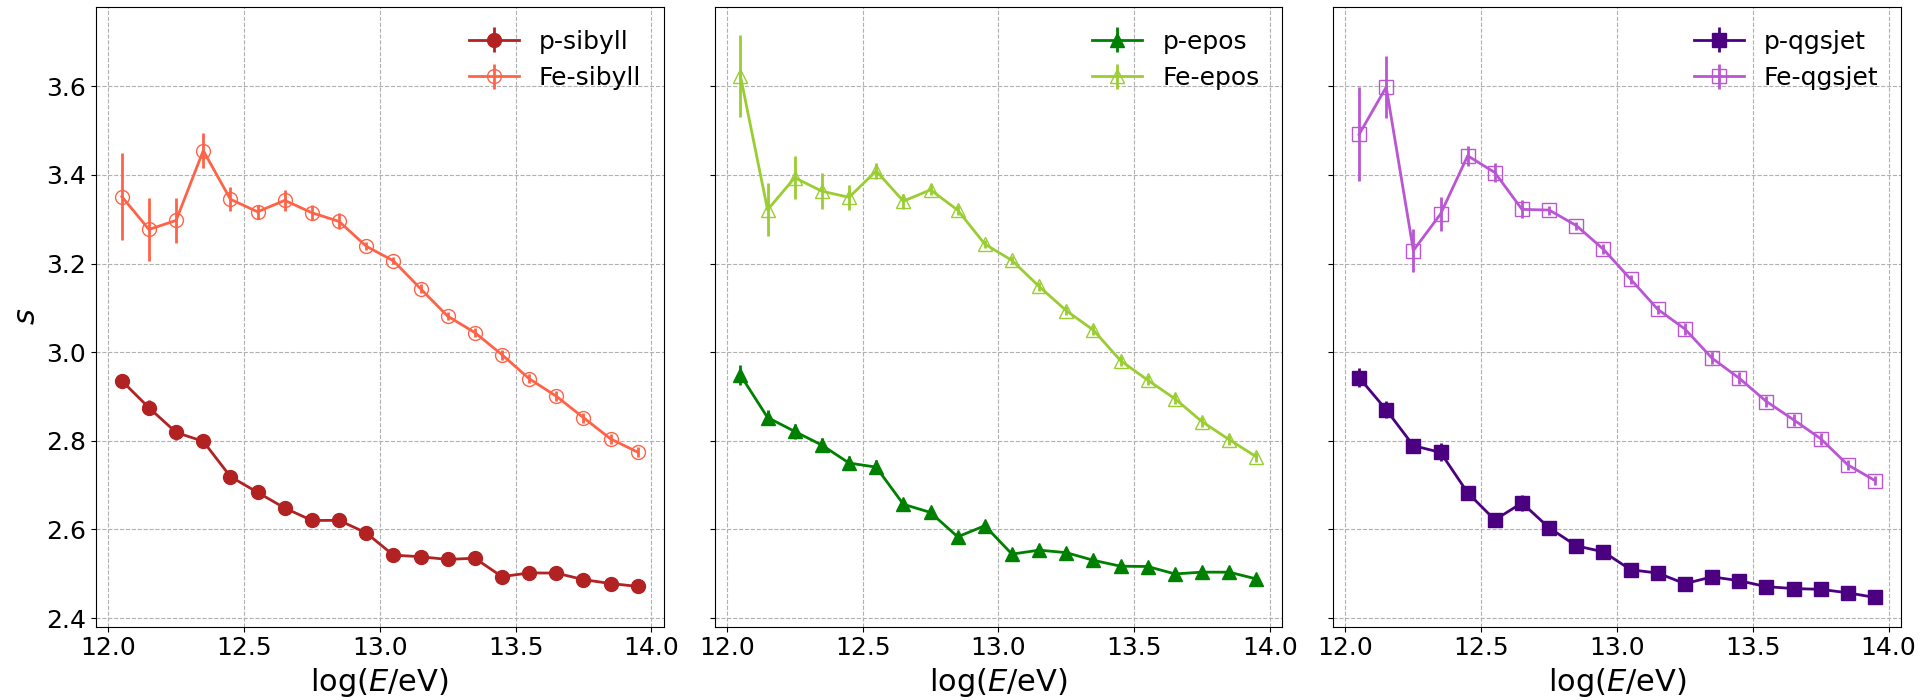
\includegraphics[width=\textwidth]{Figuras/composition_nkgs}
		\caption{Se superponen los resultados del par\'ametro $s$ para cascadas de protones y hierro. Estas \'ultimas presentan mayores valores de $s$, aludiendo a una mayor edad de las cascadas de Fe.}
		\label{fig:composition_nkgs}
		\end{figure}	
%	\ccnote{Comparaci\'on entre A y s obtenidos con diferente part\'icula primaria. (Figuras \ref{fig:composition_nkgA} y \ref{fig:composition_nkgs})}
%	\ccnote{Por qu\'e se interceptan las curvas de A????}
	
	\subsection{\'Angulo de incidencia}
%	\ccnote{Explicar diferencias entre las cascadas verticales y las m\'as inclinaditas. (Figuras \ref{fig:theta_nkgA} y \ref{fig:theta_nkgs})}
	Se simularon cascadas atmosf\'ericas con \'angulo zenital $\theta$ entre $0$ y $45^{\circ}$. Para poder analizar el efecto de $\theta$ sobre la distribuci\'on lateral de muones, el intervalo se ha dividido en dos subintervalos: $0^{\circ}<\theta<20^{\circ}$ (cascadas verticales) y $20^{\circ}<\theta<45^{\circ}$ (cascadas inclinadas). En general, una cascada inclinada atraviesa mayor cantidad de materia en la atm\'osfera que su contraparte vertical, en consecuencia al llegar al suelo est\'a m\'as avanzada en su desarrollo. Por lo mismo, al pasar m\'as atm\'osfera hay mayores p\'erdidas de energ\'ia en el medio, implicando que el n\'umero de part\'iculas de la cascada es menor. \\
	
	En las Figuras \ref{fig:theta_nkgA} y \ref{fig:theta_nkgs} se grafican los resultados de los par\'ametro $A$ y $s$, respectivamente, habiendo realizado independientemente los ajustes a la funci\'on \ref{eq:nkg} para las cascadas de ambos subintervalos. El comportamiento de las curvas individuales es similar a los resultados de todo el intervalo que se reportan en secciones anteriores. En la gr\'afica del par\'ametro $A$ se observa que efectivamente la curva resultante de las cascadas verticales est\'a por encima de la correspondiente a las inclinadas, coincidiendo con la idea de que en una cascada inclinada estar\'ian presentes menor cantidad de part\'iculas, afectando la componente hadr\'onica y por consiguiente al n\'umero de muones a nivel del suelo. \\
		\begin{figure} [h]
		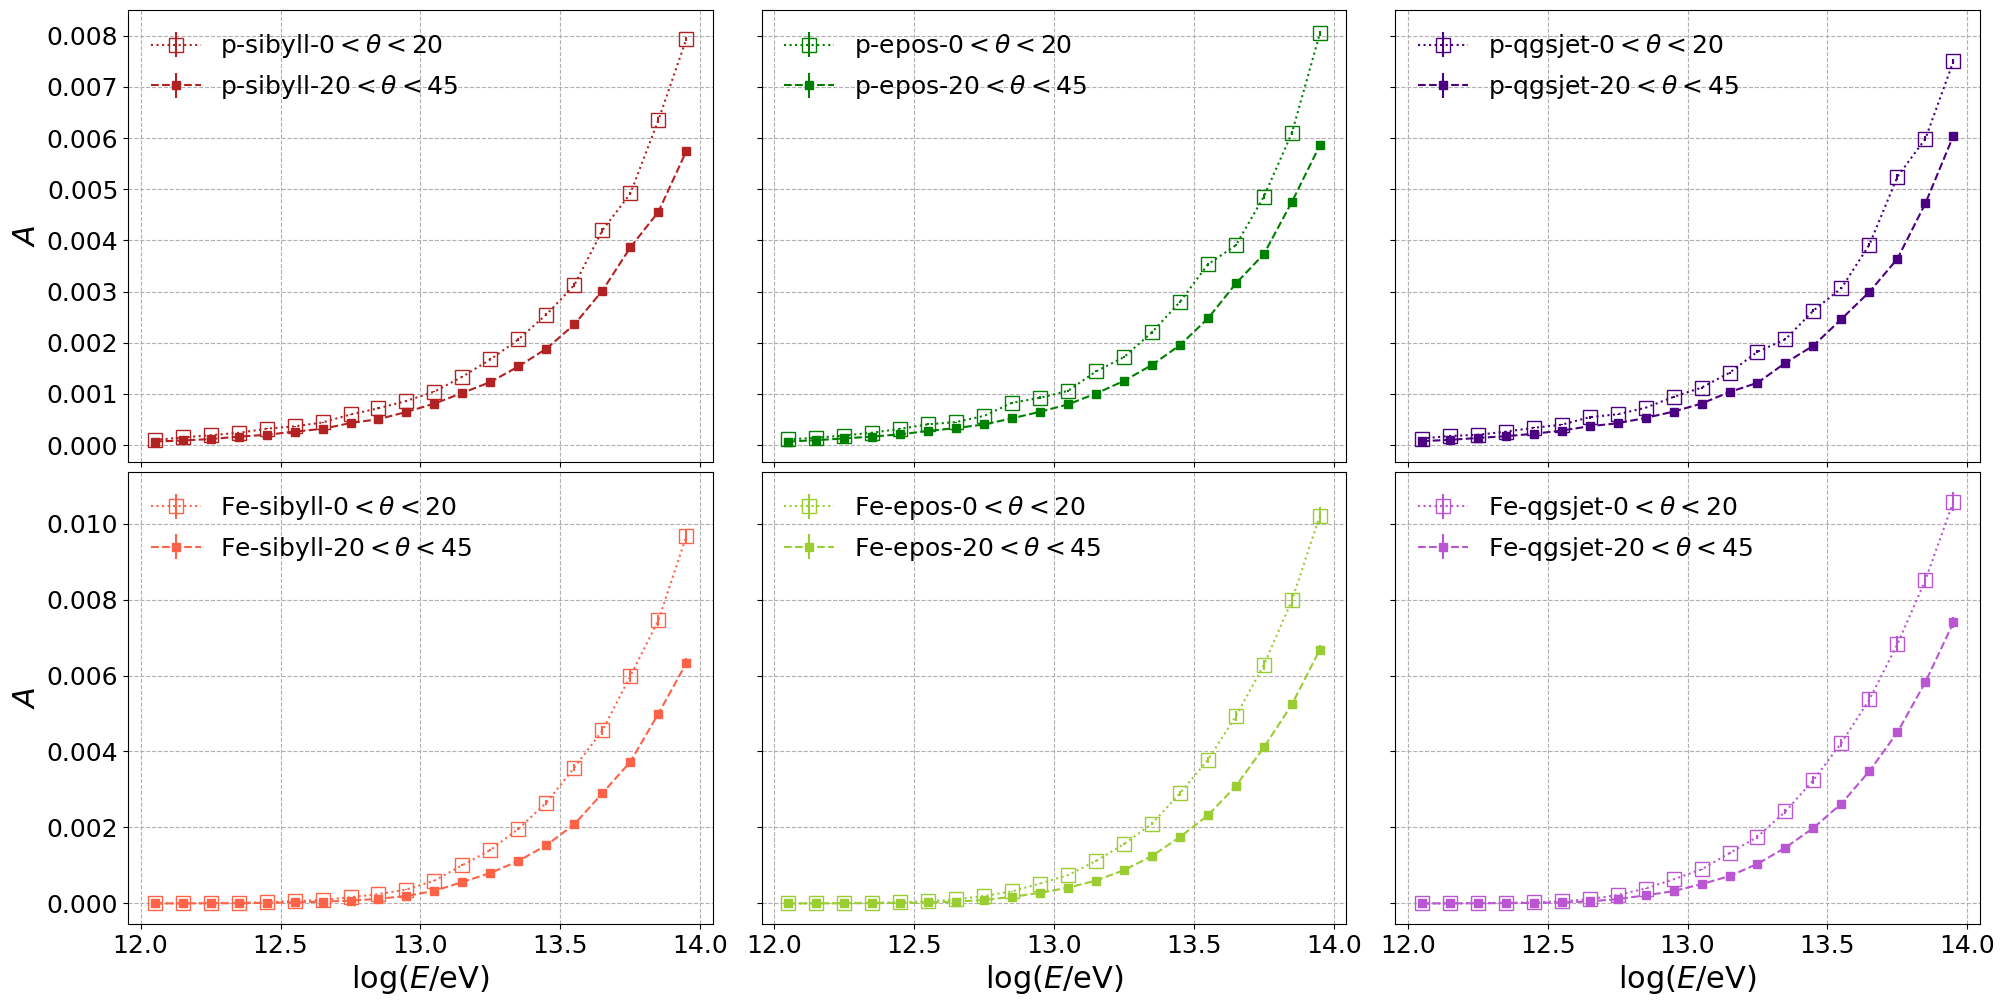
\includegraphics[width=\textwidth]{Figuras/theta_nkgA}
		\caption{Resultados del par\'ametro $A$, segmentando el grupo de cascadas en verticales e inclinadas. A partir de $E=10^{13}$ eV, se ve que los valores $A$ para las cascadas verticales son mayores que para las inclinadas, esto debido a la menor cantidad de materia que debe atravesar.}
		\label{fig:theta_nkgA}
		\end{figure}
		
		\begin{figure} []
		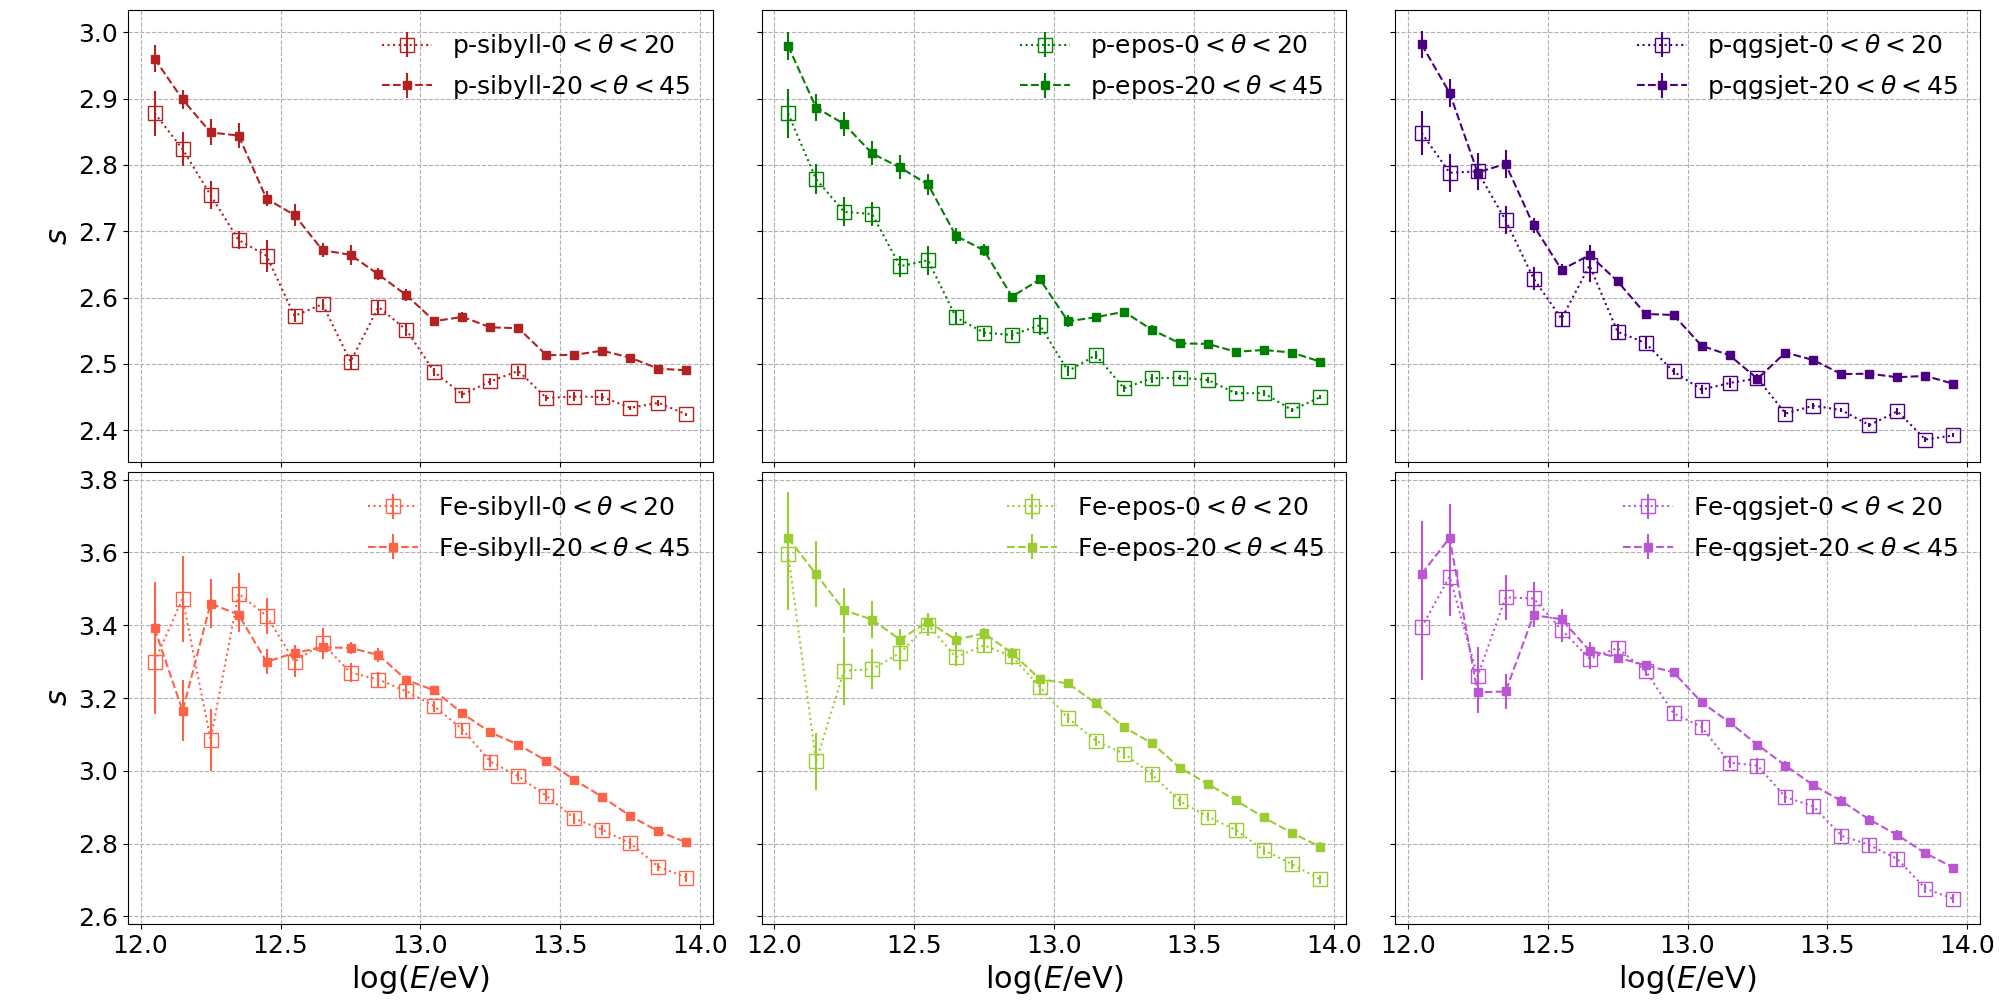
\includegraphics[width=\textwidth]{Figuras/theta_nkgs}
		\caption{Resultados del par\'ametro $s$ en cascadas verticales e inclinadas. Se observa que las cascadas m\'as desarrolladas (mayor $s$) son las verticales, sin embargo en el caso del Fe esto no es evidente hasta energ\'ias $>10^{13}$ eV.}
		\label{fig:theta_nkgs}
		\end{figure}

	Asimismo, los resultados del par\'ametro $s$ indican mayor edad para las cascadas inclinadas; en el caso de cascadas iniciadas por protones \'este es el caso para todo el rango de energ\'ia primaria, mientras que para las de hierro comienza a ser evidente a partir de los $10$ TeV, esto debido principalmente a las mayores incertezas a bajas energ\'ias. Este resultado es tambi\'en conforme a lo que se esperaba respecto al efecto del \'angulo zenital sobre el desarrollo de una cascada; al llegar al nivel del suelo las cascadas verticales son m\'as ``j\'ovenes'' que las inclinadas porque han atravesado menos atm\'osfera, y por tanto est\'an menos desarrolladas. 

\section{N\'umero de muones}
Adem\'as de las distribuciones laterales, se ha calculado una aproximaci\'on del n\'umero de muones $N_{\mu}$ que podr\'ian ser detectados en la superficie cubierta por el observatorio HAWC. El arreglo de detectores de agua Cherenkov de HAWC cubre un \'area de $22000$ m$^2$. Por simplicidad se ha supuesto que el eje de las cascadas est\'a sobre la zona central del observatorio y se ha contado $N_{\mu}$ sobre un \'area circular de $\approx 15400$ m$^2$ (radio de $70$ m). En la Figura \ref{fig:hawc} se representa esquem\'aticamente la disposici\'on de los tanques del observatorio y se indica el per\'imetro de la superficie circular para la que se calcul\'o el n\'umero de muones.\\
	\begin{figure} []
	\centering
	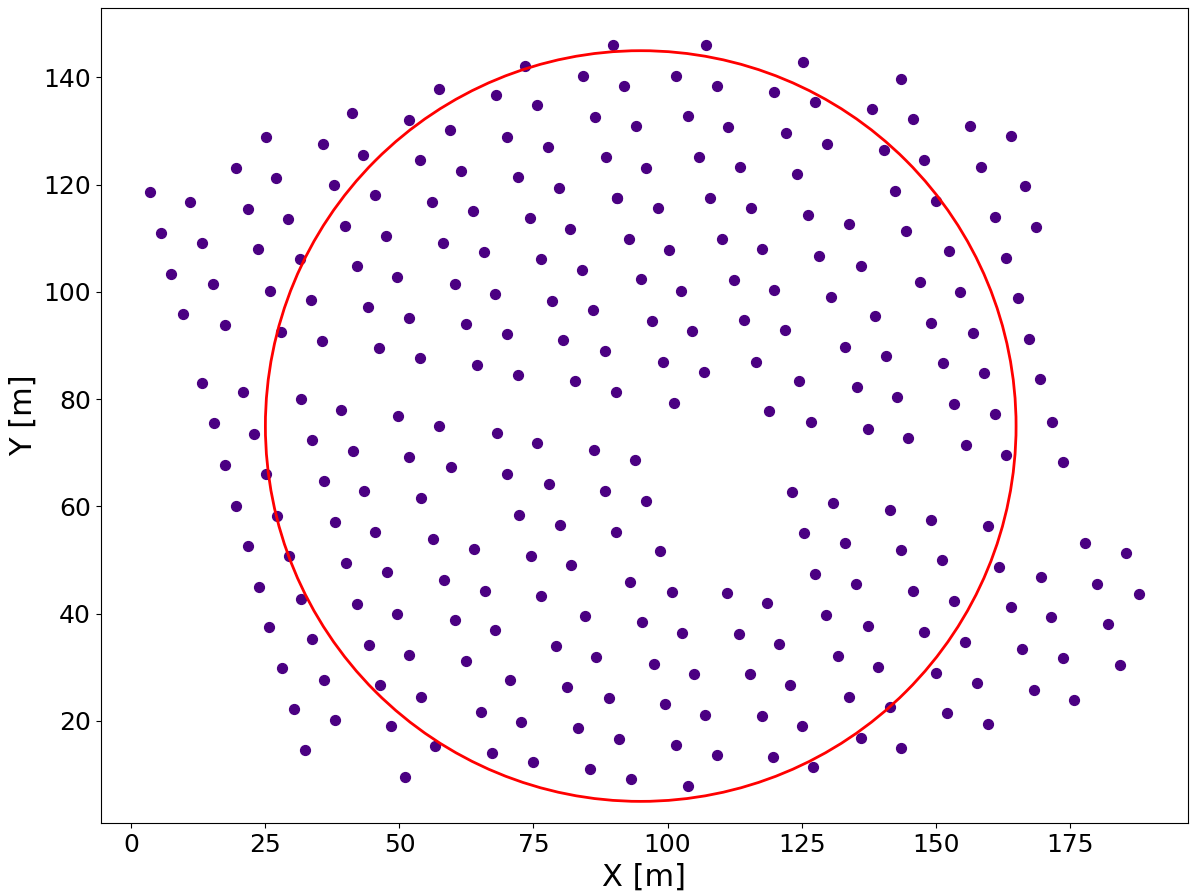
\includegraphics[width=0.6\textwidth]{Figuras/HAWC_array}
	\caption{Esquema de la disposici\'on de los detectores de agua Cherenkov que conforman HAWC. Cada punto representa un tanque. La superficie encerrada en la circunferencia roja ($R=70$ m) es el \'area utilizada para calcular un aproximado del n\'umero de muones producidos en cascadas atmosf\'ericas que podr\'ian detectarse en el observatorio.}
	\label{fig:hawc}
	\end{figure}

En primer lugar se extrajo el n\'umero de muones con $r<70$ m directamente de los resultados de las simulaciones. Posteriormente, se calcul\'o el n\'umero de muones a partir de la funci\'on \ref{eq:nkg} de la forma
	\begin{align} \label{eq:nkg_Nmu}
	N_{\mu} = 2 \pi \int_0^R r \rho_{\mu}(r) \dd{r},
	\end{align}
con $R=70$ m. Se observa en la Figura \ref{fig:munumbers} que calculando $N_{\mu}$ a partir de la funci\'on de $\rho(r)$ de tipo NKG, con los par\'ametros que se obtuvieron del ajuste, se consiguen n\'umeros menores que los que produce la simulaci\'on, siendo m\'as notorio a partir de una energ\'ia primaria de $\approx 32$ TeV.\\	
	\begin{figure} []
	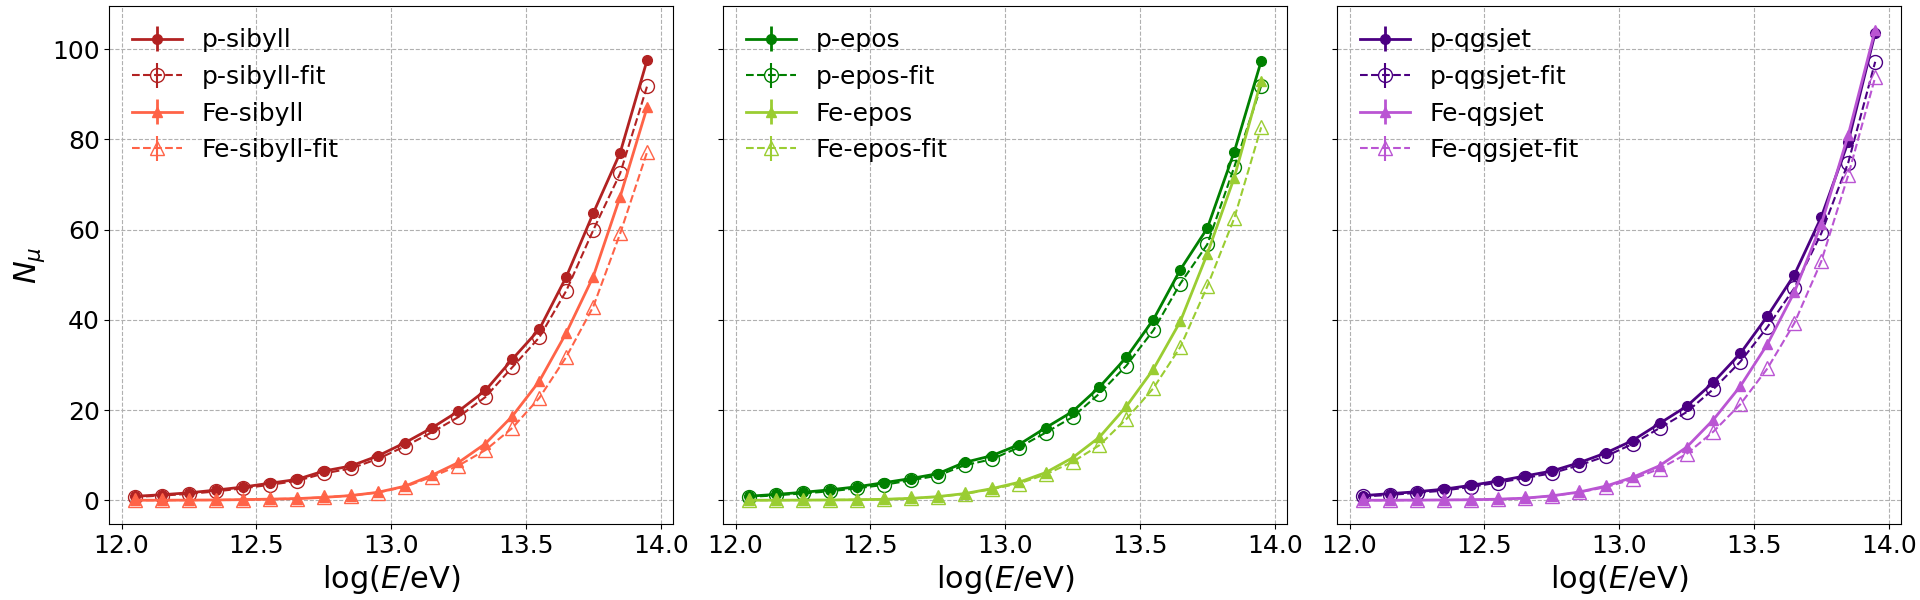
\includegraphics[width=\textwidth]{Figuras/munumbers}
	\caption{N\'umero de muones que podr\'ian detectarse en HAWC. Se exponen los resultados directos de las simulaciones (l\'ineas s\'olidas y marcadores rellenos) y los resultados de integrar num\'ericamente la funci\'on de tipo NKG (\ref{eq:nkg}) (l\'ineas discontinuas y marcadores vac\'ios). En el c\'alculo se obtiene menor n\'umero de muones.}
	\label{fig:munumbers}
	\end{figure}
	
	\begin{figure} []
	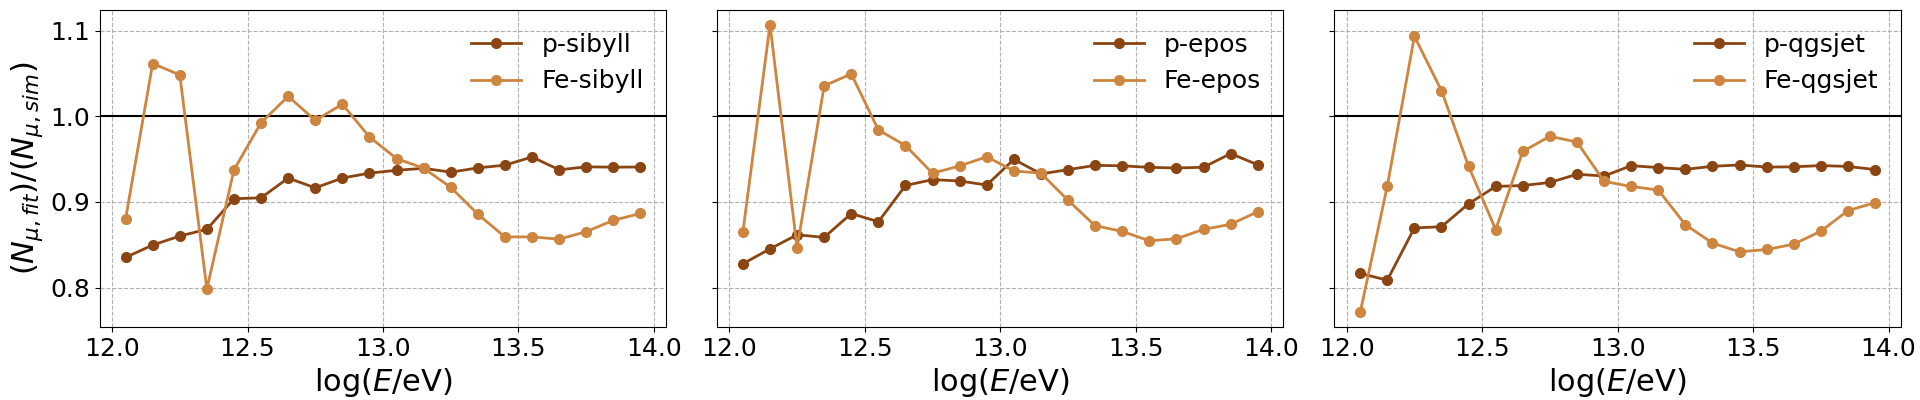
\includegraphics[width=\textwidth]{Figuras/munumbers_ratios}
	\caption{Razones entre $N_{\mu,fit}$, el n\'umero de muones  calculado num\'ericamente con la ecuaci\'on \ref{eq:nkg_Nmu} a partir del ajuste y $N_{\mu,sim}$, el n\'umero de muones obtenido directamente de las simulaciones.}
	\label{fig:munumbers_ratios}
	\end{figure}
	
Como una medida de qu\'e tan bien ajusta la funci\'on de tipo NKG a los valores que se han extra\'ido de AIRES, en la Figura \ref{fig:munumbers_ratios} se muestran las razones entre los resultados de los ajustes y los resultados de las simulaciones, donde se confirma que utilizando la ecuaci\'on \ref{eq:nkg_Nmu} se obtienen, en general, menores valores de $N_{\mu}$. En promedio, los errores del ajuste relativos a los valores simulados son aproximadamente 9\% para las cascadas de protones y 10\% para las de hierro, mientras que los valores m\'aximos de error los presenta el modelo QGSJET con 19\% y 23 \%  respectivamente para cascadas de protones y de n\'ucleos de hierro.
	
\singlespacing